\chapter{About}
The primary goal of the project is to create a new platform for exploring, presenting, and supporting European visual art in virtual space.

Our vision emphasizes sustainability and leverages cutting-edge technologies like AI, virtual reality, and blockchain for long-term development.
Audience

The project caters to European visual artists, creators, galleries, collectors, curators, visitors, and art enthusiasts. Main focus: European visual art encompassing fine arts, photography, street art, video, etc.

\section{Innovations}

\subsection[3D]{Spatial 3D Gallery Environment}
The game like 3D environment allows artists to create their own exhibitions in a virtual space, providing a unique and immersive experience for visitors. The platform offers a variety of gallery environments to choose from, each with its own distinct style and atmosphere, enabling artists to curate their exhibitions in a space that complements their artwork.

For galleries and museums, the platform offers the possibility to create digital twins of their physical spaces or design entirely new digital environments for exhibitions, opening up new opportunities for showcasing art and engaging with audiences in innovative ways.

\subsection[NFT]{NFT Integration for Gallery Presentation}
The rise of digital art traded as NFTs has created a new market landscape, dominated by a few platforms like OpenSea. This project aims to bridge the gap between web3 NFT collections and traditional art, ensuring a seamless experience for both artists and digital gallery visitors.
AI Integration for Art Recognition and Browsing

\subsection[AI]{AI features for securing Art and improving the Browsing Experience}
The integration of advanced AI technology now facilitates the incorporation of smart tools capable of recognizing and categorizing art pieces. These tools significantly enhance the user experience by seamlessly navigating through extensive artistic collections and galleries. Users benefit from additional guidance and suggestions provided by the AI, streamlining the exploration process and enriching their interaction with art.
Referential implementation overview

Referential implementation integrates the minimum basic functionality of the virtual gallery environment.

\section{Target Audience}
The prototype accommodates the general functionality flows based on the user type and further decomposed in the requirements section:

\begin{itemize}
    \item \textbf{Visitors:}
        \begin{itemize}
            \item User-friendly experience emphasizing art presentation
            \item Public access to a diverse range of European art
            \item AI virtual assistant for discovering new art and staying updated on favorite artists and genres
        \end{itemize}
    \item \textbf{Artists:}
        \begin{itemize}
            \item Assembling of 3D virtual spaces for showcasing the art
        \item Utilization of blockchain technology for NFT digital art inclusion
        \end{itemize}
    \item \textbf{Galleries:}
        \begin{itemize}
            \item Creation of 3D digital twins or entirely new digital spaces for exhibitions
            \item Initial partnership with 1 main gallery in each member state, totaling 27 galleries initially
        \end{itemize}
\end{itemize}

\chapter{Features}

\section{Virtual Exhibitions}
Implementation of a 3D virtual gallery environment that allows artists to create and curate exhibitions in a digital space. The exhibitions can be customized with various gallery environments, providing a unique and immersive experience for visitors using a standard web browser. The exhibitions are viewed as an isolated environment within a browser and emulates a private exhibition experience without other visitors.
    \begin{itemize}
        \item \textbf{Spatial 3D web browser exhibitions:} The platform supports both NFT and non-NFT art, allowing artists to create mixed displays in a custom gallery prepared 3D environment. 
    \end{itemize}


\section{Blockchain Integration}
Implementation of the integration mechanism for the blockchain and NFT based art with the classical art world using novel technological approaches to art presentation and distribution. The blockchian extends the possibilities for artists to better present their art in front of a wider audience, as well as offer a new way of monetizing their work.

    \begin{itemize}
        \item \textbf{Wallet Integration:} Artists can connect their wallets to existing accounts or use them as primary accounts.
        \item \textbf{NFT art storage} Once connected, the entire NFT portfolio of the connected wallet is loaded, cached, tracked and synchronized with the Gallery account.
    \end{itemize}

\section{Art Theft Protection}
Implementation of a multi-layered approach to safeguarding artists' work, including:

    \begin{itemize}
        \item \textbf{Nightshade:} A cutting-edge technique~\cite{shan2024nightshade} that subtly alters artwork to render it useless for AI training while maintaining visual fidelity for human viewers.
        \item \textbf{NFT Minting:} Using blockchain technology to create NFTs for each artwork, ensuring verifiable authenticity and ownership.
        \item \textbf{Metadata Integration:} Leveraging standardized metadata formats to store essential information about the artwork, including artist attribution, ownership details, and licensing terms.
    \end{itemize}

\subsection{Protection from use in AI models}

Nightshade is a pioneering technique designed to protect artists' work from being exploited for training AI models. It introduces imperceptible perturbations to the image data, rendering it ineffective for AI training while preserving visual fidelity for human observers~\cite{shan2024nightshade}. This approach ensures that the artwork remains visually appealing and unaltered for human consumption, while effectively "poisoning" the data for AI algorithms.

\begin{figure}[ht]
    \centering
    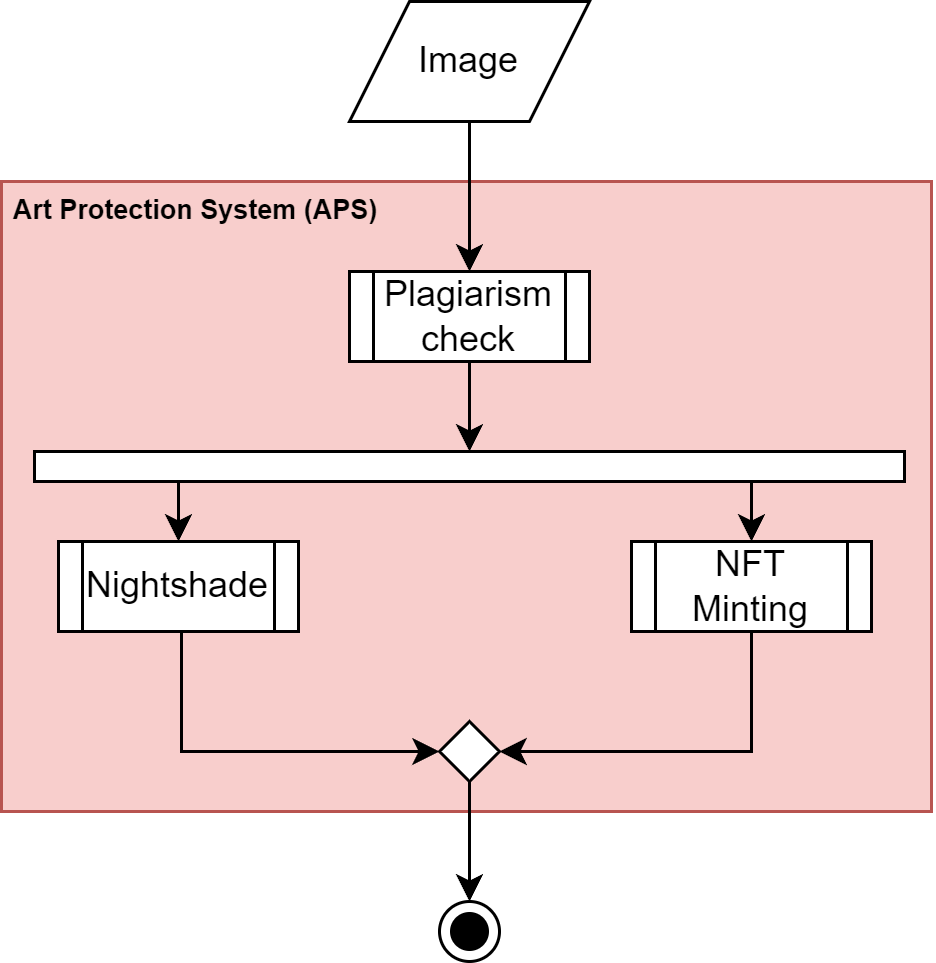
\includegraphics[width=0.8\textwidth]{figs/aps.png}
    \caption{Data flow through the processes for the Art Protection System in EVA Gallery.}
    \label{fig:data_flow}
\end{figure}

A similar tool, Glaze, focuses on protecting against style theft by subtly altering artwork to disrupt AI models' ability to mimic an artist's unique style~\cite{shan2023glaze}. However, Nightshade and Glaze are not yet interoperable, limiting their combined effectiveness in protecting against both content and style theft. EVA Gallery will monitor the development of these tools and integrate them when feasible to provide comprehensive protection against AI-powered art theft.

\subsection{Plagiarism check: a two-pronged approach}

EVA Gallery's plagiarism detection system employs a robust two-pronged approach to ensure the originality of uploaded artwork and protect artists' intellectual property rights, shown in~\autoref{fig:data_flow}.

\subsubsection{Embedding-based similarity check}

The first step involves converting the uploaded artwork into a high-dimensional numerical representation called an embedding. This embedding captures the semantic content of the image, including its objects, scenes, and overall meaning. The embedding is then compared against all existing embeddings in the database using efficient similarity search techniques like HNSW indexing. If an extremely close match is found, the artwork is flagged for further inspection.

\subsubsection{Gramian matrix similarity check}

Flagged images undergo a second level of scrutiny using Gramian matrix analysis. A Gramian matrix is a mathematical representation that captures the style of an image, including its textures, colors, and patterns. It is calculated from the feature maps extracted from the image by a pre-trained neural network.

Gramian matrices have been widely used in style transfer tasks, where the style of one image is transferred onto the content of another~\cite{nicolas2019improving}. However, their potential for style similarity comparison in the context of plagiarism detection is also promising. By comparing the Gramian matrix of the flagged image with those of existing artworks in the database, we can assess the degree of stylistic similarity. If a high match is found even at this stage, the artwork is flagged for human inspection.

This two-pronged approach provides a comprehensive check for plagiarism, considering both the semantic content and stylistic elements of the artwork. The embedding-based similarity check efficiently narrows down potential matches, while the Gramian matrix analysis delves deeper into the stylistic nuances to identify potential cases of plagiarism that may not be apparent from content alone.

By implementing this rigorous plagiarism detection system, EVA Gallery aims to create a fair and transparent platform where artists can showcase their work with confidence, knowing that their creations are protected from unauthorized copying and misuse.

\section{Plagiarism Protection}
Employ advanced techniques to detect and prevent plagiarism, ensuring the originality of uploaded artwork.

    \begin{itemize}
        \item \textbf{Embedding Space Lookup:} Artwork will be converted into numerical representations (embeddings) and compared within a vast database of existing art to identify potential copies or derivatives.
        \item \textbf{Gramian Matrix Similarity (Pending Research):}\footnote{Further research is needed to validate the effectiveness of this method for plagiarism detection.} A potential method that could further enhance plagiarism detection by analyzing the structural similarities between artworks.
        \item \textbf{Two-pronged Protection:} This system will guarantee that no modified artwork can be uploaded without proper attribution and permission, safeguarding artists' rights and fostering a fair creative environment.
    \end{itemize}

\section{Art Recommendation Engine}
Provide personalized recommendations to users based on their preferences and interactions with the artwork.

\begin{itemize}
    \item \textbf{Multi-Faceted Similarity:} Recommendations will consider both stylistic and content-based similarity to provide a diverse and engaging selection of artwork based on currently observed or displayed artwork.
    \item \textbf{Gramian-Based Style Recommendations:} Style-similar artwork will be evaluated using Gramian matrix similarity if proven viable.
    \item \textbf{Embedding-Based Content Recommendations:} Context-similar artwork will be displayed with respect to the typical similarity between embedded representations with MetaCLIP model.
    \item \textbf{Art Search:} Users will be able to input text that will be embedded and used to obtain images that most closely match the query.
\end{itemize}

\subsection{Embedding-based content recommendations}
EVA Gallery will take advantage of the power of image embeddings to provide content-based recommendations. By comparing the embedding of a user's observed artwork with the embeddings of other artworks in the database, we can identify pieces with similar semantic content, such as shared themes, subjects, or concepts. This enables us to recommend artworks that are similar to the currently observed artwork.

\subsection{Mixed recommendations (embeddings and Gramian matrices)}
To offer a diverse range of recommendations, we also consider a mixed approach that combines both embedding-based content similarity and Gramian matrix-based style similarity. This allows us to recommend artworks that share similar themes and visual styles with the observed artwork, providing a more comprehensive and engaging recommendation experience.

By incorporating both content and style information, we can cater to users who are interested in exploring artworks with similar subjects but different styles, or vice versa. This approach enhances the discovery aspect of the platform, exposing users to a wider array of artistic expressions.

\subsection{Gramian-based style recommendations}
For users who are primarily interested in visual styles, we offer recommendations based solely on Gramian matrix similarity. This allows us to identify artworks that share similar textures, colors, and patterns with the user's liked pieces, regardless of their semantic content.

This feature is particularly useful for users who are seeking inspiration for their own artistic creations or who are interested in exploring different artistic styles within a specific genre. By focusing on visual similarity, we can provide recommendations that corresponds best with the currently displayed artwork.

\chapter{User Stories}
Given the referential user types defined in the general overview, the expected user stories for the E.V.A. Gallery are:

\section{Website}
    \begin{itemize}
        \item The website should be optimized for speed and simplicity
        \item The website should use privacy non-intrusive storage to not force GDPR compliant pop ups
        \item The website is dynamically optimized for all device sizes (smartphone, tablet, laptop, large screen)
        \item The landing page contains the project logo
        \item The landing page contains a login option
        \item The landing page contains a search input
        \item The landing page contains an example query in the search input
        \item The exhibitions are rendered in browser
    \end{itemize}

\section{Visitor}
    \begin{itemize}
        \item The visitor access should not require login
        \item The visitor can access and browse individual art pieces directly or by URL
        \item The visitor can access and browse any artist collection directly or by URL
        \item The visitor can access and browse any gallery exhibition directly or by URL
        \item The visitor can view an artist profile with linked art, collections and exhibitions
        \item The visitor can search for an exhibition by its name
        \item The visitor can create an artist account to unlock the artist facing functionality
        \item The visitor's clicks and art browsing is recorded and used for further recommendations on the website
        \item The visitors are lightly fingerprinted to avoid overtraining the recommendation engine
    \end{itemize}

\section{Artist}
    \begin{itemize}
        \item The artist functionality is only available to registered users after login
        \item The artist can decide to have own account deleted
        \item The artist can create a public gallery exhibition
        \item The artist can remove own public gallery exhibition
        \item The artist can store and view own art items
        \item The artist can upload digital media representing the art items
        \item The artist can attach a web3 wallet to load NFTs
        \item The artist can choose any of the gallery environments to create an exhibition
        \item The artist can create multiple different exhibitions in the same gallery space each carrying a unique exhibition name
        \item The artist must assign a unique name to each exhibition in order to save it
        \item The artist can edit the exhibition once it is published
        \item The artist can delete the exhibition once it is published
    \end{itemize}


\chapter{Workflows}
\section{Data pipeline: Image upload and processing workflow}

Upon uploading an image to EVA Gallery, the system generates its embedding using the MetaCLIP model. This embedding captures the semantic content of the image and serves as the primary basis for content-based similarity search and recommendations.

The generated embedding is compared against all existing embeddings in the vector database using efficient similarity search techniques like HNSW indexing. If a close match is found, indicating potential plagiarism, the system extracts a Gramian matrix from either the encoded representation feature maps or from pre-computed matrices stored in the database. This Gramian matrix is then compared against the Gramian matrix of the uploaded image to assess the degree of stylistic similarity. If a high match is detected, the image is flagged for human review to determine whether it constitutes plagiarism. This and the whole pipeline is visualized in~\autoref{fig:pipeline}.

\begin{figure}[ht]
    \centering
    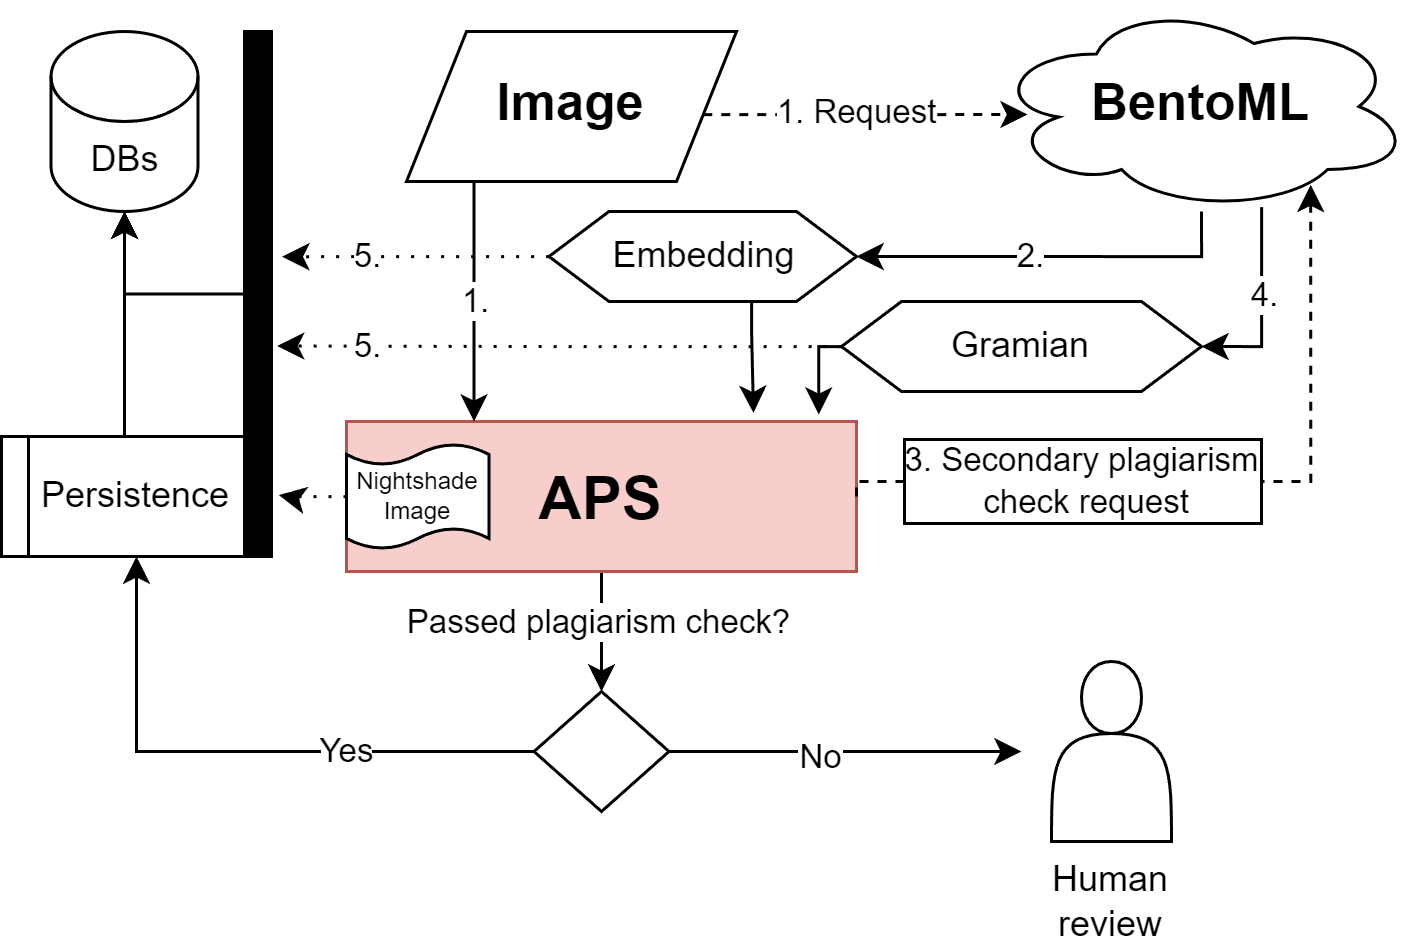
\includegraphics[width=0.8\textwidth]{figs/integ.png}
    \caption{Integration schema of the data pipeline, in other words, the image flow through the connected components of the system and the related infrastructure.}
    \label{fig:pipeline}
\end{figure}

Images that pass the plagiarism check are stored in the database along with their corresponding embeddings and Gramian matrices. Additionally, relevant metadata, including artist attribution, ownership details, and licensing terms, is associated with the image.

The artist has the option to mint the uploaded artwork as an NFT. The image is also processed with Nightshade, introducing subtle perturbations to render it useless for AI training while preserving visual fidelity. The Nightshade-processed image is stored as a separate copy in the database, linked to the original image via its unique UUID. This modified image is then displayed in the gallery, ensuring that visitors interact with the protected version while the original remains secure.

\chapter{System Requirements}
\section{AI}
\begin{enumerate}
\item \textbf{Database Access:}
    \begin{itemize}
    \item Access to a database of existing images (UUID identified).
    \item Storage for modified images (Nightshade) alongside originals.
    \end{itemize}
\item \textbf{Vector Database:}
    \begin{itemize}
    \item Storage for embeddings and Gramian matrices.
    \item HNSW indexing for efficient similarity search.
    \end{itemize}

\item \textbf{Cloud Backend:}
    \begin{itemize}
    \item Hosts MetaCLIP (embeddings) and ResNet (Gramian matrices) models.
    \item Supports batched input.
    \item Simple API (e.g., BentoML).
    \end{itemize}

\item \textbf{Hardware Requirements:}
    \begin{itemize}
    \item MVP: GPU with at least 24GB VRAM.
    \item Deployment: Scalable GPU compute with load balancing and in-flight batching
    \end{itemize}
\end{enumerate}

\section{NFT}
\begin{enumerate}
    \item \textbf{Database Access:}
    \begin{itemize}
    \item Access to a database of existing images (UUID identified).
    \end{itemize}

\item \textbf{RPC provider:}
    \begin{itemize}
    \item Access to a RPC provider for the selected chain to fetch data from.
    \end{itemize}

\item \textbf{IPFS:}
    \begin{itemize}
    \item IPFS node where the NFT contents are typically located.
    \end{itemize}
\end{enumerate}

\section{Website}
\begin{enumerate}
    \item \textbf{Database Access:}
    \begin{itemize}
    \item Access to a database of existing images (UUID identified).
    \end{itemize}

\item \textbf{Frontend:}
    \begin{itemize}
    \item Scalable provider with frontend hosting capabilities.
    \item WASM support for 3D rendering.
    \end{itemize}

\item \textbf{Backend:}
    \begin{itemize}
    \item Scalable provider with backend hosting capabilities.
    \item Connectability for other services in the project.
    \item OAUTH enabled access
    \end{itemize}
\end{enumerate}

\chapter{Technology stack}
\section{AI}

\begin{enumerate}
\item \textbf{Database Access:}
    \begin{itemize}
        \item \textbf{PostgreSQL:} A robust open-source relational database management system, offering support for structured data, ACID compliance, and scalability. Ideal for storing image metadata and maintaining associations between original and modified images.
        \item \textbf{Redis:} Local caching functionality for the frontend and backend, ensuring fast access to frequently accessed data.
    \end{itemize}

\item \textbf{Vector Database:}
    \begin{itemize}
        \item \textbf{pgvector+pgvectorscale+cube:} A PostgreSQL extension adding support for vector data types with similarity search using indexing algorithms, and matrix storage and search with cube. Cost-effective and scalable for storing and searching embeddings and Gramian matrices.
    \end{itemize}

\item \textbf{Cloud Backend:}
    \begin{itemize}
        \item \textbf{BentoML:} A flexible framework for building and deploying machine learning services. Simplifies packaging and deployment of models, allowing easy integration with various cloud providers, and supports batched input processing and API generation.
        \item \textbf{Self-hosted:} Kubernetes provides control and flexibility in configuring the software environment and automating deployment and building. We can utilize our existing servers with a proper MLDevOps architecture to ensure CI and CD alongside AI models.
        \item \textbf{IPFS instance:} Interactions with the NFT data stored in the Inter-Planetary FileSystem.
    \end{itemize}

\item \textbf{Scalable GPU Compute:}
    \begin{itemize}
        \item \textbf{Nvidia Triton Inference Server:} A high-performance inference server optimized for serving deep learning models. Supports dynamic batching and model ensemble, maximizing GPU utilization and throughput. Integrates with Kubernetes for seamless scaling and management.
    \end{itemize}
\end{enumerate}

% \chapter{API Specifications}
% \section{Backend}

% \section{NFT}
% \begin{enumerate}
%     \item \textbf{RPC Provider:}
%     \begin{itemize}
%         \item \textbf{Ethereum:} Infura, Alchemy, or similar providers for Ethereum-based chains.
%         \item \textbf{Polygon:} Alchemy, QuickNode, or similar providers for Polygon-based chains.
%     \end{itemize}

%     \item \textbf{IPFS:}
%     \begin{itemize}
%         \item \textbf{IPFS HTTP API:} IPFS HTTP API for interacting with the IPFS node, including adding and retrieving NFT contents.
%     \end{itemize}

%     \item \textbf{Functionality:}
%     \begin{itemize}
%         \item abc
%     \end{itemize}
% \end{enumerate}
% \section{AI}

\chapter{Milestone 2: Current state of progress}
This chapter addresses the project's current state and plans for the initial launch of EVA Gallery in the alpha/beta state. It will outline the features that are currently planned to be included and which are to be excluded initially, and the reasons for those decisions.
\section{Frontend}
% TODO: Add the current state of the frontend
\section{Backend}
% TODO: Add the current state of the frontend
% admin.controller.ts

\section{NFT}

\section{Eva Gallery - NFT Module}
\subsection{Choosing network for NFT infrastructure}
The NFT (Non-Fungible Token) market has experienced significant growth in recent years, attracting artists, collectors, and investors worldwide. However, this booming industry is not without its challenges, particularly in the realm of infrastructure. The current landscape of NFT technology is primarily dominated by the Ethereum network, which, despite its popularity, presents certain limitations that are becoming increasingly problematic as the market expands.

One of the most pressing issues facing the NFT market on the Ethereum network is the high gas fees associated with minting and trading NFTs. Gas fees are the costs required to perform transactions on the Ethereum blockchain, which can fluctuate based on network congestion. These fees can be prohibitively expensive for smaller artists and collectors, making it difficult for them to participate in the market. As a result, there has been a growing interest in alternative networks that offer lower fees and faster transaction times.

Several blockchain networks have emerged as potential alternatives to Ethereum, each with advantages and disadvantages. The most notable options include:

\begin{itemize}
    \item \textbf{Polygon\footnote{Polygon \url{https://polygon.technology/}}:} A layer 2 scaling solution for Ethereum, offering low fees and fast transactions.
    \item \textbf{Gnosis chain\footnote{Gnosis chain \url{https://www.gnosis.io/}}:} A new blockchain network that aims to provide low fees and fast transactions for NFTs.
    \item \textbf{Polkadot\footnote{Polkadot \url{https://polkadot.network/}}:} A multi-chain network that aims to provide low fees and fast transactions for NFTs.
    \item \textbf{Solana\footnote{Solana \url{https://solana.com/}}:} A high-performance blockchain network that offers low fees and fast transactions.
\end{itemize}

Each of these networks offers unique features and capabilities, and the choice of which network to use can depend on a variety of factors. Our initial consideration was mostly focused on EVM-based Blockchains, however, we later also added Polkadot, a promising network that stands out due to its potential for future scalability. Polkadot is designed as a multi-chain network, meaning it can handle multiple blockchains within its ecosystem, offering the potential for significantly higher transaction throughput. One of the key differences between Polkadot and EVM chains is the wallet address system. Polkadot uses a different format for wallet addresses, which may be less familiar to users accustomed to Ethereum’s system. This could present a learning curve for those new to the network.

Numerous articles and research papers compare the best blockchain networks for NFTs. For example, articles such as \cite{nfts} provide an overview of the different networks available, while research papers like \cite{fintech1030017} delve into the technical aspects and performance metrics of these networks.

To make a precise and accurate decision about which network is best suited for a particular use case, it is essential to consider several key factors:

\begin{itemize}
    \item Scalability of the network
    \item Availability of the tooling for NFT implementation and interaction with blockchain
    \item Programming language of the tooling
    \item Costs associated with creating collections and minting NFTs
    \item Speed of transactions
    \item Community support and adoption of NFT technology
    \item Environmental impact of the network
\end{itemize}

These factors are crucial because they directly influence the usability, efficiency, and sustainability of an NFT platform. For instance, scalability refers to the network's ability to handle a large number of transactions without significant delays or increased costs. Tooling availability is also important as it determines how easy it is for developers to create and manage NFTs on the network. The programming language used by the tooling is another consideration, as it affects the accessibility and flexibility of the development process.

Costs are always a significant concern, particularly for smaller artists or collectors who may be priced out of the market by high fees. Transaction speed is equally important, as faster transactions improve user experience by reducing waiting times. Community support and adoption are critical for ensuring that there is a robust ecosystem of users, developers, and marketplaces that can support and drive the growth of NFTs. Lastly, the environmental impact of the network is an increasingly important consideration, as concerns about the carbon footprint of blockchain technology continue to grow.

We have compared these factors across all the mentioned networks, as shown in two separate Tables \ref{tab:networks} \& \ref{tab:networks2}.

\begin{table*}[htb!]
    \caption{Comparison of various selected Blockchain Network parameters and NFT infrastructure part I.}
\centering
\small
\begin{tabular}{|l|l|l|l|l|}
\hline
Network      & Scalability                                                                                                                                                                                                   & Tooling                                                                                                  & Prog. lang.                                                    & Avg. per NFT        \\ \hline
Ethereum     & \begin{tabular}[c]{@{}l@{}}Often overloaded\\ when something \\ popular is released\\ (Drives GAS fees \\ up). 15-30 TPS \\ throughtput.\end{tabular}                                                         & \begin{tabular}[c]{@{}l@{}}ERC721A \\ standard \\ for cost \\ optimization\end{tabular}                  & \begin{tabular}[c]{@{}l@{}}Solidity,\\ Javascript\end{tabular} & $\sim$$10 - $100+\$   \\ \hline
Polygon      & \begin{tabular}[c]{@{}l@{}}Created as ETH\\ L2 chain to offlift\\ ETH. \\ $\sim$65000 TPS\end{tabular}                                                                                                        & \begin{tabular}[c]{@{}l@{}}Crossmint API\\ for collection \\ and nft \\ mint abstraction\end{tabular}    & \begin{tabular}[c]{@{}l@{}}Solidity,\\ Javascript\end{tabular} & $\sim$$0.01 - $0.05\$ \\ \hline
Gnosis chain & \begin{tabular}[c]{@{}l@{}}L2 solution hosted\\ by over 215.000\\ active validators\\ $\sim$155 TPS\end{tabular}                                                                                              & \begin{tabular}[c]{@{}l@{}}GoldRush to get\\ NFTs associated \\ with account\end{tabular}                & \begin{tabular}[c]{@{}l@{}}Solidity,\\ Javascript\end{tabular} & $\sim$$0.10 - $0.50\$ \\ \hline
Polkadot     & \begin{tabular}[c]{@{}l@{}}As multichain \\ network Polkadot \\ is able to disperse \\ transactions to\\ different chains \\ (Up to 300 chains \\ can be in one \\ network) \\ $\sim$100.000 TPS\end{tabular} & \begin{tabular}[c]{@{}l@{}}Substrate \\ framework,\\ PolkadotJS \\ libraries\end{tabular}                & \begin{tabular}[c]{@{}l@{}}Rust,\\ Javascript\end{tabular}     & $\sim$$0.006-$0.01\$   \\ \hline
Solana       & \begin{tabular}[c]{@{}l@{}}Solana aims to be\\ one of the most \\ scalable blockchains \\ when it comes to \\ TPS \\ $\sim$65000 TPS\end{tabular}                                                             & \begin{tabular}[c]{@{}l@{}}Compressed \\ NFTs - Minting \\ 1.000 NFTs \\ should cost 300\$.\end{tabular} & Rust, C                                                        & $\sim$$3 - $4\$       \\ \hline
\end{tabular}
    \label{tab:networks}
    \end{table*}

\begin{table*}[htb!]
    \caption{Comparison of various selected Blockchain Network parameters and NFT infrastructure part II.}
\centering
\small
\begin{tabular}{|l|l|l|l|}
\hline
Network      & Block processing time & NFT adoption                                                                                                                                                     & Env. impact                                                                                                              \\ \hline
Ethereum     & $\sim$12 seconds      & \begin{tabular}[c]{@{}l@{}}Very popular,\\ hosts some of \\ the most expensive \\ collections ever \\ made\end{tabular}                                          & \begin{tabular}[c]{@{}l@{}}After migrating\\ to PoS consensus\\ 99\% less\\ $\sim$2.8 kilotonnes\\ per year\end{tabular} \\ \hline
Polygon      & $\sim$2.1 seconds     & \begin{tabular}[c]{@{}l@{}}Significantly lesser\\ adoption compared\\ to ETH, downtrend \\ in NFT adoption\end{tabular}                                          & \begin{tabular}[c]{@{}l@{}}$\sim$60.9 tonnes \\ per year\end{tabular}                                                    \\ \hline
Gnosis chain & $\sim$5 seconds       & \begin{tabular}[c]{@{}l@{}}Infrastructure strongly\\ tied to PoaPs, other\\ collections hardly\\ present\end{tabular}                                            & \begin{tabular}[c]{@{}l@{}}$\sim$25 tonnes\\ per year\end{tabular}                                                       \\ \hline
Polkadot     & $\sim$12 seconds      & \begin{tabular}[c]{@{}l@{}}NFT infrastructure\\ well built but not\\ as utilized. Uses\\ different wallet \\ addresses (32B \\ compared to EVM 20B)\end{tabular} & \begin{tabular}[c]{@{}l@{}}$\sim$33 tonnes \\ per year\end{tabular}                                                      \\ \hline
Solana       & $\sim$0.6 seconds     & \begin{tabular}[c]{@{}l@{}}NFT adoption on\\ very strong level,\\ some collections\\ have more than \\ 130.000.000 eur \\ total volume\end{tabular}              & \begin{tabular}[c]{@{}l@{}}$\sim$8.875 tonnes\\ per year\end{tabular}                                                    \\ \hline
\end{tabular}
    \label{tab:networks2}
    \end{table*}

Tables \ref{tab:networks} \& \ref{tab:networks2} provides a comprehensive comparison of various blockchain networks and their suitability for NFT infrastructure. While Ethereum remains the most popular choice due to its widespread adoption and extensive documentation, it also has the highest gas fees and slower transaction times. This makes it less accessible for smaller creators and collectors who may be discouraged by the high costs associated with using the Ethereum network.

Polygon, as an Ethereum layer 2 solution, offers significantly lower fees and faster transactions. However, despite its technical advantages, it has seen a downtrend in NFT adoption, possibly due to its lesser degree of decentralization compared to Ethereum. The NFT infrastructure on Polygon, although functional, does not appear to be maturing at the same pace as on Ethereum.

Gnosis Chain is another alternative, which, while offering low fees and faster transactions, still lacks the community support and widespread adoption seen on other networks. Its NFT infrastructure is closely tied to Proof of Attendance Protocols (PoAPs), but beyond that, the variety and popularity of NFT collections on Gnosis Chain are limited.

Polkadot presents an interesting case with its multi-chain network architecture, allowing for high scalability. However, the network’s use of a different wallet address format and its still-developing ecosystem may be hurdles for broader adoption, especially among users who are already familiar with Ethereum-based systems. Despite these challenges, Polkadot’s ability to support on-chain NFT minting without the need for extensive smart contract development could be a significant advantage as the network grows.

Solana, a high-performance blockchain with very low fees and rapid transaction times, is gaining traction within the NFT community. Its innovative approach to NFT creation, particularly through the use of compressed NFTs, makes it an appealing option for large-scale projects. Additionally, Solana's commitment to eco-friendliness, with one of the lowest carbon footprints among blockchain networks, positions it as a sustainable choice for the future.

After careful consideration of the facts mentioned above, we decided to choose Kusama (Polkadot's canary network) mainly because of the NFT minting which happens on-chain lifting developers from creating and auditing smart contracts for NFT distribution. The price to mint NFT is among the lowest compared to other chains. As the ecosystem is slowly growing we can expect, that the NFT adoption will rise as well. The tooling seems to also be sufficient enough for EVA Galery use cases.

\subsection{NFT-Module infrastructure breakdown}
The Non-Fungible Token (NFT) Module provides a set of endpoints that allow users to create collections or non-fungible assets within a blockchain environment. This document provides a comprehensive overview of the main endpoints used to interact with the NFT Module, including the creation of individual NFTs and collections, as well as transferring ownership of NFTs.

The NFT Module offers several key endpoints that enable interaction with NFT assets and collections. Below is a detailed explanation of each endpoint, including examples of JSON bodies that can be used when making requests.

\subsubsection{PUT /collection/\{id\}/asset}
This endpoint is used to generate an NFT based on the parameters provided in the request body. The NFT is created within a specific collection, identified by the \texttt{id} parameter in the URL.

\begin{itemize}
    \item \textbf{URL:} \texttt{/collection/\{id\}/asset}
    \item \textbf{Method:} PUT
\end{itemize}

\subsubsection{Example JSON Body}
\begin{lstlisting}[language=json]
{
    "metadata": {
        "name": "Example asset name",
        "description": "Example asset description",
        "ipfs": "IPFS image link",
        "author": "address"
    }
}
\end{lstlisting}

\subsubsection{Explanation}
The JSON body must include the metadata for the NFT:
\begin{itemize}
    \item \texttt{name}: The name of the NFT.
    \item \texttt{description}: A brief description of the NFT.
    \item \texttt{ipfs}: The IPFS link pointing to the image or media associated with the NFT.
    \item \texttt{author}: The address of the creator of the NFT.
\end{itemize}

\subsection{PUT /collection}
This endpoint is used to generate a new NFT collection based on the parameters provided in the request body.

\begin{itemize}
    \item \textbf{URL:} \texttt{/collection}
    \item \textbf{Method:} PUT
\end{itemize}

\subsubsection{Example JSON Body}
\begin{lstlisting}[language=json]
{
    "owner": "address",
    "metadata": {
        "name": "NFT name",
        "description": "NFT description",  // Optional
        "ipfs": "IPFS image link" // Optional
    }
}
\end{lstlisting}

\subsubsection{Explanation}
The JSON body for creating a collection includes:
\begin{itemize}
    \item \texttt{owner}: The address of the collection owner.
    \item \texttt{metadata}: An object containing:
    \begin{itemize}
        \item \texttt{name}: The name of the collection.
        \item \texttt{description}: An optional description of the collection.
        \item \texttt{ipfs}: An optional IPFS image link associated with the collection.
    \end{itemize}
\end{itemize}

\subsection{POST /transfer/collection/\{collection\}/asset/\{asset\}}
This endpoint facilitates the transfer of ownership of a non-fungible asset from one address to another.

\begin{itemize}
    \item \textbf{URL:} \texttt{/transfer/collection/\{collection\}/asset/\{asset\}}
    \item \textbf{Method:} POST
\end{itemize}

\subsubsection{Example JSON Body}
\begin{lstlisting}[language=json]
{
    "address": "13TrdLhMVLcwcEhMYLcqrkxAgq9M5gnK1LZKAF4VupVfQDUg"
}
\end{lstlisting}

\subsubsection{Explanation}
The JSON body requires the \texttt{address} field, which represents the new owner's address.

\subsection{GET /address/\{address\}}
This endpoint retrieves all NFTs owned by the specified address on the Kusama network.

\begin{itemize}
    \item \textbf{URL:} \texttt{/address/\{address\}}
    \item \textbf{Method:} GET
\end{itemize}

\subsubsection{Explanation}
This GET request does not require a body, only the \texttt{address} URL parameter to specify the address whose NFTs are to be retrieved.

\subsection{Implementation Example}
Below is an example of how to implement a fetch request to create an NFT asset using the \texttt{PUT /collection/\{id\}/asset} endpoint.

\subsubsection{JavaScript Fetch Request Example}
\begin{lstlisting}[language=Javascript]
const response = await fetch("http://localhost:3000/collection/1/asset", {
    method: 'PUT',
    headers: {
        'Content-Type': 'application/json'
    },
    body: JSON.stringify({
        "metadata": {
            "name": "Example asset name",
            "description": "Example asset description",
            "ipfs": "IPFS image link",
            "author": "13TrdLhMVLcwcEhMYLcqrkxAgq9M5gnK1LZKAF4VupVfQDUg"
        }
    })
});
const resp = await response.json();
\end{lstlisting}

\subsubsection{Explanation}
In the example above, the fetch request sends a PUT request to create a new NFT within a collection with ID 1. The metadata for the NFT, including its name, description, IPFS link, and author address, is passed in the request body.

\subsection{Response and Hex Encoding}
All PUT and POST endpoints return a HEX encoded call, which must be passed to the back-end (BE) system that then returns them to the front-end for signing. The front-end will prompt the signer to sign the transaction. Below is an example of a HEX encoded call returned after calling the create an NFT endpoint:

\begin{lstlisting}
"0x71020428020834030100000002000000006cf3e7bf1cc5f0b87e7aaa8
bc5acf2489651b14e768bcf5d9206f878778f44040034180100000002000
00081017b226e616d65223a224578616d706c65206173736574206e616d6
5222c226465736372697074696f6e223a224578616d706c6520617373657
4206465736372697074696f6e222c2269706673223a224950465320696d6
16765206c696e6b227d"
\end{lstlisting}

\subsubsection{Explanation}
When decoded, the above HEX string translates into a batch of calls required to create the NFT. The decoding process reveals the JSON structure of the calls that were made. Decoded call can be observed in figure \ref{hex}.

\begin{figure}[h!]
    \centering
    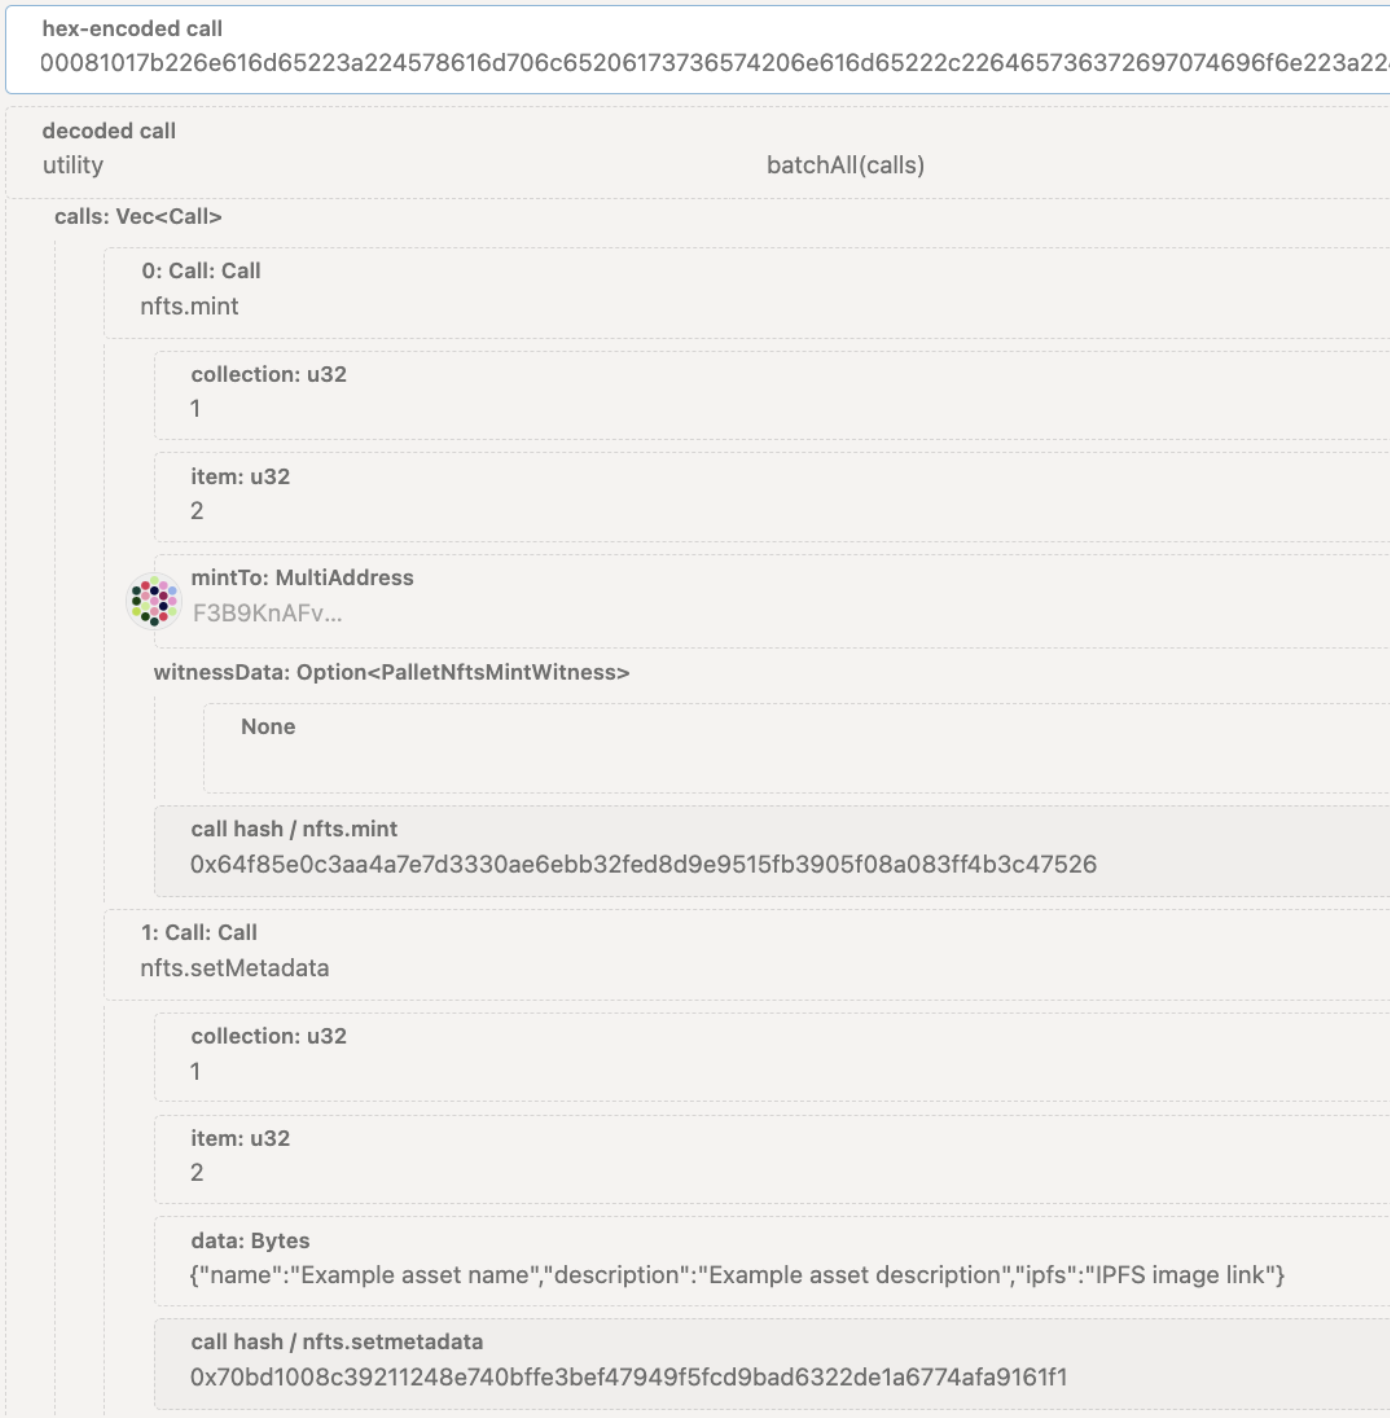
\includegraphics[width=\textwidth]{figs/nft-decoded-extrinsic.png}
    \caption{Decoded batch of calls}
    \label{hex}
\end{figure}

\section{Next steps - NFT Module}
The NFT module is currently being integrated into the back end of the Eva Gallery application. This process involves several key updates and enhancements to ensure seamless functionality for managing NFTs within the platform.

Firstly, the database infrastructure requires an upgrade to support the storage of NFT Asset metadata. This involves creating new database schemas and tables designed to handle the unique properties of NFTs, such as their ownership details, and metadata associated with each digital asset (e.g., titles, descriptions, and creator information). The data architecture must be optimized for efficiency and scalability, given the potential volume of NFTs that the application may host.

In parallel, an image IPFS (InterPlanetary File System) uploading mechanism needs to be developed. The IPFS is a decentralized storage solution that ensures the assets associated with NFTs, like images or videos, are stored in a distributed manner, enhancing security and reducing the risk of data loss. This involves integrating the IPFS protocol into the back-end, enabling users to upload digital files that are then hashed and stored on the IPFS network. These files are linked to the corresponding NFT metadata in the database, ensuring that each NFT is fully traceable and verifiable.

The front end is required to enable users to interact with their cryptocurrency wallets directly through the Eva Gallery interface. Their wallet will be able to connect through the wallet connect component. This will enable various functionalities, such as viewing NFT holdings, initiating transactions, and managing ownership within the platform.

Additionally, the transaction signing process needs to be integrated into the front-end interface. This involves assigning transaction prompts to specific user actions within the application. For instance, when a user clicks on the "Mint artwork as NFT" button, the system should trigger a wallet prompt requesting the user to sign the transaction. This ensures that all operations requiring blockchain interaction—such as minting or transferring are securely authorized by the user.

Together, these upcoming changes will enable the Eva Gallery application to fully support NFT functionality, providing users with a seamless experience for creating and managing NFTs within a secure and decentralized Blockchain environment.
\textbf{Polkadot} was chosen as the target blockchain due to the combination of low fees, fast transactions, and a growing NFT ecosystem. 

\subsection{Implementation}
The integration with the previously selected blockchain was performed.

\begin{description}
    \item[Wallet Integration:] Infrastructure of the backend allows the artists to connect the wallet and load the onchain asset information into the backend module for further processing.
    \item[NFT art storage:] Stubbed implementations allowing calling the external IPFS service to load the content of the metadata referenced digital art.
\end{description}

\section{AI}

As we prepare for the initial launch of EVA Gallery in its alpha/beta state, the following key features have been prioritized for inclusion:

\begin{description}
    \item[Ability to Find Similar Images Based on Currently Viewed Image:] Users are able to easily discover visually similar artwork by utilizing a feature that identifies and suggests images related to the one currently being viewed. This capability leverages advanced image recognition and comparison algorithms.
    \item[AI-Powered Image Search:] The search functionality within EVA Gallery will be enhanced by embedding both text queries and images into a shared vector space. This allows users to perform more intuitive and accurate searches, finding artworks that match their textual descriptions or visual preferences.
    \item[Embedding-Based Plagiarism Detection:] To protect artists’ intellectual property, the platform will include an embedding-based plagiarism detection system. This system converts artwork into numerical embeddings and compares them against a database to identify potential copies or derivatives, ensuring that the originality of artwork is preserved.
    \item[NoAI and NoTrain Meta Tags:] EVA Gallery will implement NoAI and NoTrain meta tags within its site metadata. These tags will serve as signals to scraping bots, indicating that the site’s content is off-limits for AI training purposes. This proactive measure will help protect the artwork from being exploited by AI models without consent.
    item[Other Scraping Protections:] In addition to meta tags, EVA Gallery will employ various other scraping protection techniques to prevent unauthorized data extraction. These protections will be part of a broader strategy to safeguard artists' work and maintain the integrity of the platform.
\end{description}

\noindent
The following features will instead be excluded due to time constraints or limitations outside of our control, for the alpha/beta launch:

\begin{description}
    \item[Nightshade and Glaze AI-Training Protection:] While these tools offer promising methods for preventing AI models from using protected artwork, their implementation requires access to specific model weights that are not currently publicly available. We have contacted the authors of these tools and are awaiting their response. Until these resources are accessible, these protections cannot be integrated into the platform.
    \item[Gramian-Based Similarity and Search:] This advanced feature, which involves using Gramian matrices to evaluate and search for stylistic similarities between artworks, remains theoretical and unproven. Further research and validation are needed before it can be included in EVA Gallery's feature set. As such, it will not be available in the initial launch but may be considered for future updates.
\end{description}